%----------- Capítulo 3: Especificação do Software -------------

\chapter{Especificação do Software}
% TODO: talvez seja bom mudar o nome desse capítulo para Especificação e Arquitetura do software
% vide http://pt.wikipedia.org/wiki/Processo_de_desenvolvimento_de_software
O software em questão consiste em um serviço web que tem como principal funcionalidade responder a rota entre dois pontos informados com menor tempo de viagem utilizando o sistema de transporte público. 
Nas subseções a seguir são apresentados os requisitos do sistema bem como o projeto de sua arquitetura.

\section{Requisitos do Sistema}
O primeiro passo para o desenvolvimento de qualquer sistema computacional é levantar seus requisitos. 
A seguir estão listados os requisitos funcionais e não-funcionais do sistema proposto.

\subsection{Requisitos Funcionais}
Os requisitos funcionais visam levantar informações a respeito do sistema proposto quanto às suas funcionalidades, ou seja, é o serviço que se espera fornecer ao usuário final.
A seguir encontra-se a lista completa de requisitos funcionais deste projeto. 

Quanto à interface do sistema:
\begin{itemize}
	\item O software deverá retornar para o usuário a rota com menor tempo de viagem entre dois pontos informados.
	\item O software deverá mostrar a rota resultante desenhada em um mapa, diferenciando as linhas de transporte por cor, e também no formato texto como uma sequência de passos.
	\item O software deverá receber do usuário os pontos de partida/destino no formato de endereço ou marcando-os no mapa.
	\item O sistema deverá ser acessado através de um navegador web.
\end{itemize}

\subsection{Requisitos Não-Funcionais}
Os requisitos não-funcionais referem-se a aspectos não-funcionais do sistema, como restrições nas quais o sistema deve operar.
Estes são disponibilizados a seguir.

Quanto a distribuição do software:
\begin{itemize}
	\item O software deverá ser disponibilizado como livre, possibilitando futuras contribuições.
	\item O software deverá ser disponibilizado no formato de um serviço web.
	\item O software 
\end{itemize}

Quanto à fonte de dados:
\begin{itemize}
	\item O software deverá funcionar independente de qual fonte de dados for escolhida, contudo que esta respeite o padrão GTFS.
	\item O software deverá utilizar um banco de dados de grafos para armazenamento das rotas do sistema de transporte público.
	\item O software deverá ter seu banco de dados populado com um mínimo de informações sobre as rotas do serviço de transporte público, sendo estas:
	\begin{itemize}
		\item As rotas existentes no serviço de transporte público.
		\item As paradas ou estações existentes.
		\item Horários de chegada e partida de veículos de cada parada ou estação.
		\item As coordenadas geográficas de cada parada ou estação.
	\end{itemize}
\end{itemize}

Quanto às ferramentas:
\begin{itemize}
	\item O sistema gerenciador de banco de dados deverá responder à consultas rapidamente.
	\item O software deverá ser hospedado em um servidor que suporte todas as ferramentas computacionais utilizadas.
\end{itemize}


\section{Arquitetura do Sistema}
O sistema em questão é composto de quatro núcleos principais: \emph{Core, GTFS Importer, Web Service} e um Cliente. 
O projeto de fluxo padrão do sistema como um todo é mostrado na figura \ref{fig:arquitetura}.

\begin{figure}[!htb]
	\centering
	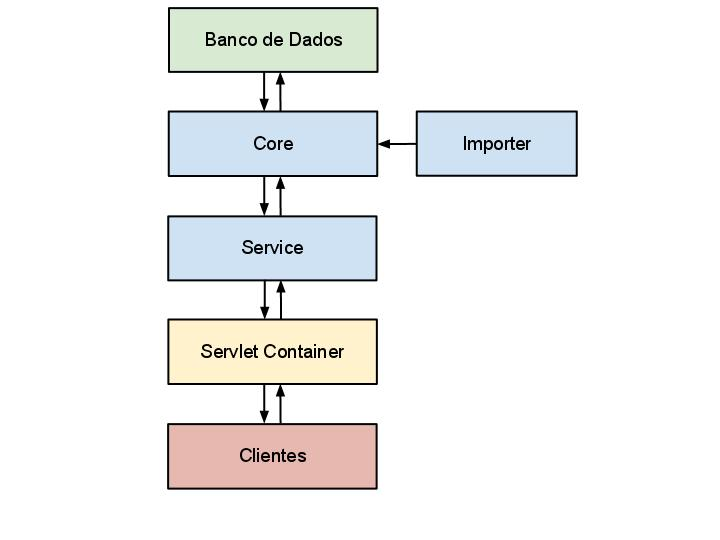
\includegraphics[width=0.6\textwidth]{./arquitetura.jpg}
	\caption[Arquitetura do sistema]{Visão geral da arquitetura do sistema.}
	\fonte{Autoria Própria}
	\label{fig:arquitetura}
\end{figure}

Primeiramente o usuário informa os pontos de origem e destino para o Cliente marcando-os no mapa disponibilizado ou fornecendo o endereço por extenso nas devidas caixas de texto, juntamente com o horário de partida da origem.
Feito isso, os dados coletados são enviados ao \emph{Web Service} para que este execute uma busca no banco de dados. 
Esta busca é realizada através das funcionalidades contidas no \emph{Core} do sistema e tem como objetivo encontrar a rota de caminho mínimo entre os pontos informados.
Ao terminar de executar a \emph{query} no banco, o \emph{Web Service} responde ao Cliente as informações sobre a rota resultante sendo estas por fim mostradas ao usuário de duas formas: uma sequência de passos em formato texto e um desenho da rota no mapa.

Para que qualquer consulta seja bem sucedida, é necessário que o banco de dados esteja populado com as informações dos arquivos no padrão GTFS, esta a qual é realizada através do núcleo \emph{GTFS Importer}.
A seguir uma explicação detalhada de cada módulo do sistema.

\subsection{Core}
Este módulo foi projetado para conter todas as representações das entidades que compõem o sistema, bem como suas respectivas \emph{factories} e um controle de acesso ao banco de dados.
O diagrama de projeto do pacote \emph{Core} é mostrado na figura \ref{fig:core}.

\begin{figure}[!htb]
	\centering
	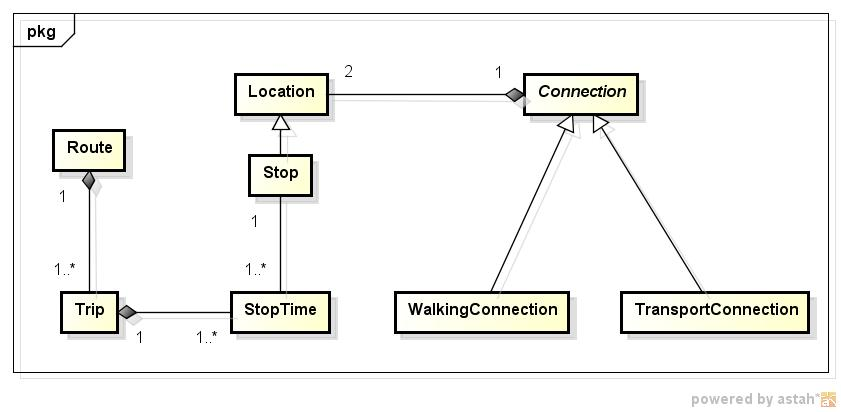
\includegraphics[width=1\textwidth]{./CoreDiagram.jpg}
	\caption[Arquitetura do Core]{Visão geral da arquitetura do Core.}
	\fonte{Autoria Própria}
	\label{fig:core}
\end{figure}

Como se pode observar, o \emph{Core} é composto pelas seguintes entidades especificadas no padrão GTFS:

\begin{itemize}
	\item \textbf{Route}: contém informações a respeito de uma linha de transporte público, tais como o nome da rota, o meio de transporte utilizado, e as \emph{Trips} que a compõem.
	\item \textbf{Trip}: é uma sequência de duas ou mais entidades \emph{StopTime}, ou seja, dois ou mais pontos de parada de embarque/desembarque que ocorrem em um certo instante de tempo determinado.
	\item \textbf{Location}: consiste em um ponto de coordenadas geográficas e suas respectivas conexões de entrada e saída.
	\item \textbf{Stop}: um tipo de \emph{Location} que consiste em um ponto de parada de veículos para entrada e saída de passageiros.
	\item \textbf{StopTime}: contém informações de horários de partida e chegada de veículos em uma determinada \emph{Stop} pertencente a uma \emph{Trip}.
	\item \textbf{Connection}: consiste em uma conexão entre dois pontos, contendo informações tais como a distância e o custo de tempo entre a origem e destino. 
	Uma \emph{Connection} pode ser do tipo \emph{TransportConnection} e \emph{WalkingConnection}, sendo que a primeira consiste em uma conexão entre duas entidades \emph{Stop} e a segunda entre uma \emph{Stop} e uma \emph{Location}.
\end{itemize}

Para a criação no sistema de cada uma destas entidades foi utilizado o conceito de \emph{factories}. 
Uma \emph{factory} nada mais é que um \emph{design pattern} que consiste em uma interface para a criação de famílias de objetos correlatos ou dependentes.
Desta forma, optou-se por implementar \emph{factories} para criação de cada entidade presente no \emph{Core}.

Todas as entidades do módulo em questão são armazenados no banco de dados através da classe \emph{DatabaseController}.
Esta nada mais é que uma camada de abstração do acesso ao banco, com o objetivo de permitir uma troca do sistema gerenciador de banco de dados rapidamente caso necessário.
Além disso, é na classe \emph{DatabaseController} que se encontra o algoritmo principal do sistema para encontrar o caminho com tempo de viagem mínimo entre os pontos de origem e destino fornecidos pelo usuário.


\subsection{Importer}
Módulo responsável pela importação e mapeamento dos arquivos GTFS para o banco de dados. 
Seu principal objetivo é o de adquirir informações dos arquivos GTFS e, utilizando as \emph{factories} respectivas às entidades do \emph{Core}, mapeá-las e relacioná-las no banco de dados para grafos.
Porém, os arquivos do padrão GTFS contém muita informação opcional para o funcionamento do sistema, sendo que muitas destas nem sempre são disponibilizadas. 
Desta forma, foi definido que o mínimo de informação necessária para o funcionamento do sistema são os campos obrigatórios do padrão GTFS, os quais são citados na tabela \ref{tab:campos_obrigatorios}.

\begin{table}[!htb]
	\centering
	\caption{Campos obrigatórios importados dos arquivos GTFS para funcionamento do sistema}
	\label{tab:campos_obrigatorios}
	\begin{tabular}{ll}
		\hline
		\textbf{Arquivo} & \textbf{Campos Obrigatórios} \\
		\hline
		\textbf{Route} & \emph{route ID}: identifica um trajeto \\
				    & \emph{short name}: nome abreviado de um trajeto \\
				    & \emph{long name}: nome completo de um trajeto \\
		\textbf{Trip} & \emph{trip ID}: identifica uma viagem \\ 
				& \emph{route ID} \\ 
				& \emph{service ID}: identifica a disponibilidade do serviço por data \\
		\textbf{Stop} & \emph{stop ID}: identifica uma parada ou estação \\
				 & \emph{name}: nome de uma parada ou estação \\
				 & \emph{latitude, longitude}: coordenadas geográficas da parada ou estação \\
		\textbf{StopTime} & \emph{trip ID} \\
				         & \emph{stop ID} \\
				         & \emph{arrival/departure time}: tempo de chegada/partida do veículo de uma parada \\
				         & \emph{stop sequence}: ordem das paradas de uma viagem \\
		\hline
	\end{tabular}
	\fonte{\cite{GTFSspecs}}
\end{table}

Sem essas informações importadas para o banco de dados o sistema é incapaz de cumprir o objetivo de responder a rota ótima entre dois pontos considerando o tempo de viagem.

\subsection{Web Service}
Este é o módulo responsável por executar a \emph{query} no banco de dados em busca do caminho de tempo de viagem mínimo entre os pontos informados pelo usuário.
 
Ao receber as coordenadas geográficas dos pontos de origem e destino do módulo Cliente, o \emph{Web Service} primeiramente cria os respectivos nós de origem e destinho no grafo através do \emph{Core}, mais especificamente com a classe \emph{DatabaseController}.
Estes nós são então conectados aos diversos pontos de parada de veículos com o custo de tempo baseado na distância e velocidade de caminhada, sendo a última uma constante definida em \emph{Constants}.
 
Com os pontos presentes no grafo, o \emph{Web Service} executa uma \emph{query} de busca de caminho mínimo. Feito isso, os pontos de origem e destino são descartados do grafo e retorna-se o resultado ao módulo Cliente.
 
\subsection{Cliente Web}
Responsável pela aquisição de dados de entrada do usuário e encaminhamento dos mesmos ao \emph{Web Service}.
Primeiramente o usuário informa o endereço de origem e destino à interface web do Cliente através de um \emph{browser}, sendo que estes são repassados em seguida ao \emph{Web Service} no formato de coordenadas geográficas, para que o mesmo busque o caminho mínimo requisitado.
É necessária uma conexão com a internet para que a busca seja realizada, já que o funcionamento do sistema baseia-se num \emph{Web Service}.
 
Ao receber resposta do \emph{Web Service}, o Cliente se responsabiliza de mostrar o resultado desenhando a rota resultante no mapa através das coordenadas geográficas dos pontos e descrevendo passo-a-passo as ações a serem tomadas para se chegar ao destino.
 
\section{Considerações}
Neste projeto do sistema procurou-se modularizar ao máximo seus componentes, de tal forma que se caso surjam modificações seja rápido e fácil de implementá-las.
Cada um dos módulos foi idealizado com base na sua funcionalidade principal visando minimizar o grau de dependência entre os mesmos, o que facilita futuros reaproveitamentos de código, contribuições ao projeto, e a própria divisão de trabalho entre os integrantes da equipe.

Em suma, os seguintes módulos foram definidos no projeto:
\begin{itemize}
	\item O \emph{Core} tem como objetivo definir todas as entidades e relações a serem armazenadas no banco de dados, bem como interfacear o acesso do sistema ao mesmo.
			Cada uma destas entidades possui sua respectiva \emph{factory}, centralizando desta forma sua criação no sistema por tipo de entidade.
			Já o interfaceamento com o banco de dados é realizado pela classe \emph{DatabaseController} e tem como objetivo tornar o sistema flexível quanto ao SGBD utilizado.

	\item O \emph{Importer} consiste basicamente em importar todas as entidades dos arquivos GTFS ao banco de dados através das funcionalidades contidas no \emph{Core}.
	\item O Cliente consiste na interface com o usuário, ou seja, coleta de informação e mostra de informações a respeito da rota resultante.
	Buscou-se flexibilizar a conexão entre o sistema e o Cliente, para que futuramente sejam desenvolvidos diferentes tipos de clientes, como por exemplo para dispositivos móveis.
	\item O \emph{Web Service} é o responsável por, com os dados fornecidos vindos do Cliente, calcular a rota de caminho mínimo através das funcionalidades do \emph{Core}.
\end{itemize}

O projeto da arquitetura do sistema tornou-se uma excelente base para o processo de implementação.
Com o mesmo foi definido detalhadamente os requisitos necessários e o que tinha que ser feito para se ter um sistema funcional, bastando somente buscar a maneira mais propícia para desenvolver o que foi idealizado.
